\textbf{Исходный текст:} \\
    Привет!

\textbf{Публичный ключ $(e, n)$:} \\
    (5491526198967652564128883404649, 8677899933955039287323181182263)

\textbf{Приватный ключ $(d, n)$:} \\
    (6530236606095563597175180039049, 8677899933955039287323181182263)

\textbf{Зашифрованный текст:} \\
    2451790758248836813047077465653 6929963014385198466056100423531
    1792994633186142959029214273249 1068251925414506252246529379223
    6486422004695066299507395395040 4941598345502762856208188833893
    6161224323360842715260972435122

Результаты работы программы представлены на рисунках~\ref{ris:encode-test-2}-\ref{ris:decode-test-2}.

\vspace{\baselineskip}
\begin{figure}[H]
\center{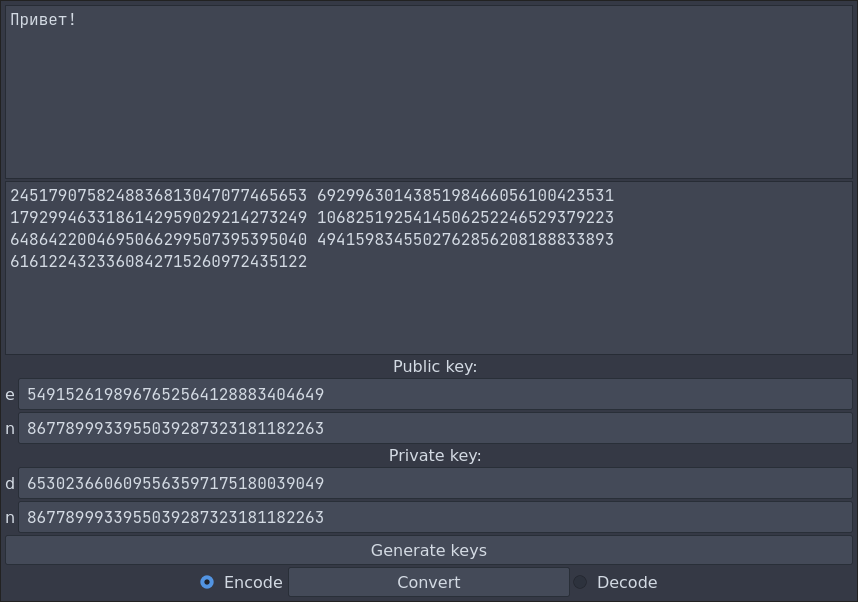
\includegraphics[width=0.8\linewidth]{figures/encode-test-2}}
    \caption{Шифрование}
\label{ris:encode-test-2}
\end{figure}

\vspace{\baselineskip}
\begin{figure}[H]
\center{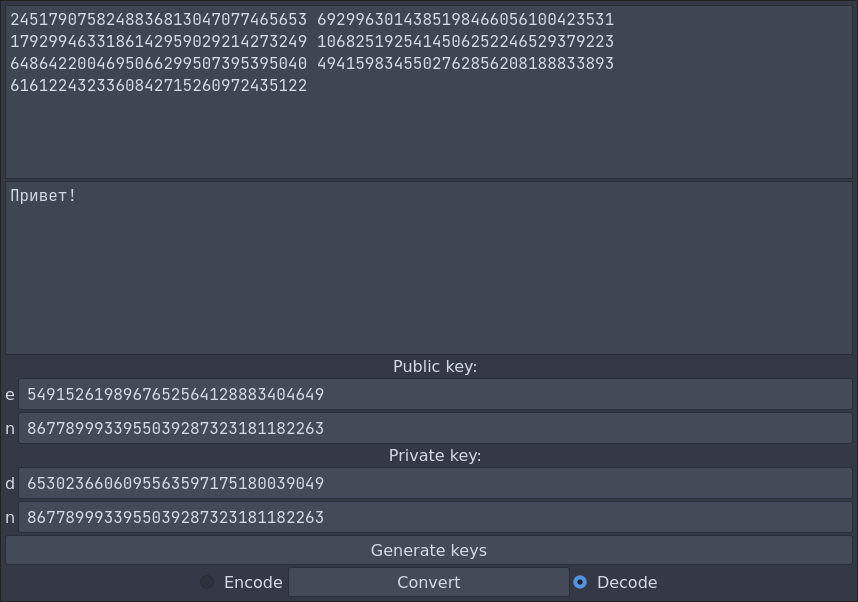
\includegraphics[width=0.8\linewidth]{figures/decode-test-2}}
    \caption{Расшифрование}
\label{ris:decode-test-2}
\end{figure}
